\documentclass[bigtut]{tutorial}\usepackage[]{graphicx}\usepackage[]{color}
%% maxwidth is the original width if it is less than linewidth
%% otherwise use linewidth (to make sure the graphics do not exceed the margin)
\makeatletter
\def\maxwidth{ %
  \ifdim\Gin@nat@width>\linewidth
    \linewidth
  \else
    \Gin@nat@width
  \fi
}
\makeatother

\definecolor{fgcolor}{rgb}{0.345, 0.345, 0.345}
\newcommand{\hlnum}[1]{\textcolor[rgb]{0.686,0.059,0.569}{#1}}%
\newcommand{\hlstr}[1]{\textcolor[rgb]{0.192,0.494,0.8}{#1}}%
\newcommand{\hlcom}[1]{\textcolor[rgb]{0.678,0.584,0.686}{\textit{#1}}}%
\newcommand{\hlopt}[1]{\textcolor[rgb]{0,0,0}{#1}}%
\newcommand{\hlstd}[1]{\textcolor[rgb]{0.345,0.345,0.345}{#1}}%
\newcommand{\hlkwa}[1]{\textcolor[rgb]{0.161,0.373,0.58}{\textbf{#1}}}%
\newcommand{\hlkwb}[1]{\textcolor[rgb]{0.69,0.353,0.396}{#1}}%
\newcommand{\hlkwc}[1]{\textcolor[rgb]{0.333,0.667,0.333}{#1}}%
\newcommand{\hlkwd}[1]{\textcolor[rgb]{0.737,0.353,0.396}{\textbf{#1}}}%
\let\hlipl\hlkwb

\usepackage{framed}
\makeatletter
\newenvironment{kframe}{%
 \def\at@end@of@kframe{}%
 \ifinner\ifhmode%
  \def\at@end@of@kframe{\end{minipage}}%
  \begin{minipage}{\columnwidth}%
 \fi\fi%
 \def\FrameCommand##1{\hskip\@totalleftmargin \hskip-\fboxsep
 \colorbox{shadecolor}{##1}\hskip-\fboxsep
     % There is no \\@totalrightmargin, so:
     \hskip-\linewidth \hskip-\@totalleftmargin \hskip\columnwidth}%
 \MakeFramed {\advance\hsize-\width
   \@totalleftmargin\z@ \linewidth\hsize
   \@setminipage}}%
 {\par\unskip\endMakeFramed%
 \at@end@of@kframe}
\makeatother

\definecolor{shadecolor}{rgb}{.97, .97, .97}
\definecolor{messagecolor}{rgb}{0, 0, 0}
\definecolor{warningcolor}{rgb}{1, 0, 1}
\definecolor{errorcolor}{rgb}{1, 0, 0}
\newenvironment{knitrout}{}{} % an empty environment to be redefined in TeX

\usepackage{alltt}
\unitcode{MATH1005}
        \unitname{Statistics}
        \semester{Summer/Winter/Semester2}
        \sheetnumber8

\usepackage{graphicx}
\withsolutions
\IfFileExists{upquote.sty}{\usepackage{upquote}}{}
\begin{document}
\lettersfirst

\begin{tutorial}

\begin{displaybox}
{\bf Linear Function of a Random Variable}  \\ 
Given a random variable $X$ with $E(X)$ and $Var(X)$. \\
For constants $a$ and $b$,  \\
 $E(a+bX) = a + bE(X)$ and $Var(a+bX) = b^2 Var(X)$. \\ \\

{\bf Sums of Random Variables}  \\ 
Given a sequence of random variables $X_i$ with $E(X_i)$ and $Var(X_i)$ for $i=1,\ldots,n$. \\
$E \Big( \sum_{i=1}^{n} X_i  \Big)    = \sum_{i=1}^{n} E(X_i)$.  \\
If  $X_i$ are independent,  $Var \Big( \sum_{i=1}^{n} X_i \Big) = \sum_{i=1}^{n} Var(X_i)$. 
\end{displaybox}

\begin{displaybox}
{\bf Sums of Normal Random Variables}  \\ 
Given a sequence of independent random variables $X_i \sim N(\mu_i, \sigma_i^2)$ for $i=1,\ldots,n$. \\
$ \sum_{i=1}^{n} a_i X_i     \sim N \Big(  \sum_{i=1}^{n} a_i \mu_i, \sum_{i=1}^{n} a_i^2 \sigma_i^2 \Big)$ \\ \\

Given a sequence of iid random variables $X_i \sim N(\mu, \sigma^2)$ and constants $a_{i}$ for $i=1,\ldots,n$  \\
$ \bar{X} = \frac{1}{n} \sum_{i=1}^{n} X_i     \sim N \Big(  \mu, \frac{\sigma^2}{n} \Big) $ \\
$ \sum_{i=1}^{n} X_i     \sim N(  n \mu, n \sigma^2)$ \\ 
\end{displaybox}

\begin{displaybox}
{\bf Central Limit Theorem (CLT)} \\

Given a sequence of iid random variables $X_i \sim ( \mu, \sigma^2) $  for $i=1,\ldots,n$. \\
where $\sigma^2 < \infty$ and $n$ is large, \\
then the distribution function of  $ \frac{ \sum_{i=1}^{n} X_i  - n \mu } { \sqrt{n \sigma^2} }$ tends  to the standard Normal. \\ 

Less formally,  
$ \sum_{i=1}^{n} X_i \rightarrow   N(  n \mu, n \sigma^2 )$ 
and  $ \bar{X} \rightarrow   N(  \mu,  \frac{ \sigma^2}{n} )$.  

\end{displaybox}


\begin{displaybox}
{\bf Normal Approximation to the Binomial (CLT special case)} \\

For large $n$, $X \sim Bin(n,p) \rightarrow N(np, np(1-p))$. \\ 

Guide: Use when $n > 25$, $np >5$, $n(1-p) > 5$.
\end{displaybox}

\begin{displaybox}
{\bf Continuity correction} \\

Given a discrete integer valued RV $X \sim (\mu, \sigma^2)$ and the approximating Normal $Y \sim N(\mu, \sigma^2)$ \\
we adjust by 1/2 to (usually) improve the approximation. \\
$ P(X \geq x) \rightarrow P(Y \geq x-1/2) $ \\
$ P(X \leq x) \rightarrow P(Y \leq x+1/2) $

\end{displaybox}


\begin{questions}

\vspace{.5cm}
\question Linear Function of a Discrete Random Variable  \\

\begin{parts}

\part Consider the following probability distribution function of $X$.

\begin{center}
\begin{tabular}{| l | l | l | l | l | l |} \hline
$x$ & 1 & 2 & 3 & 4 & Total \\ \hline
$P(X=x)$ & 0.1 & 0.2 & 0.3 &  0.4 & 1 \\ \hline
\end{tabular}
\end{center}

\begin{parts}
\item 
Show $E(X) = \sum_{i=1}^{4} x P(X=x) = 3$, $E(X^2) = \sum_{i=1}^{4} x^2 P(X=x) = 10$ and $Var(X) = 1$.

\item Check in R
\begin{knitrout}
\definecolor{shadecolor}{rgb}{0.969, 0.969, 0.969}\color{fgcolor}\begin{kframe}
\begin{alltt}
\hlstd{x}\hlkwb{=}\hlkwd{c}\hlstd{(}\hlnum{1}\hlopt{:}\hlnum{4}\hlstd{)}
\hlstd{p}\hlkwb{=}\hlstd{x}\hlopt{/}\hlnum{10}
\hlkwd{sum}\hlstd{(x}\hlopt{*}\hlstd{p)}
\hlkwd{sum}\hlstd{(x}\hlopt{^}\hlnum{2}\hlopt{*}\hlstd{p)}\hlopt{-}\hlkwd{sum}\hlstd{(x}\hlopt{*}\hlstd{p)}\hlopt{^}\hlnum{2}
\end{alltt}
\end{kframe}
\end{knitrout}
\end{parts}

\part Now consider a linear function of $X$, namely $Y=1+2X$. 

\begin{parts}
\item Complete the following probability distribution function of $Y$.

\begin{center}
\begin{tabular}{| l | l | l | l | l | l |} \hline
$y$ & 3 & &  &  & Total \\ \hline
$P(Y=y)$ & 0.1 &  \hspace{1cm} & \hspace{1cm}  & \hspace{1cm}  & 1 \\ \hline
\end{tabular}
\end{center}

\part
Find $E(Y)$ and $Var(Y)$.

\part Check in R.
\begin{knitrout}
\definecolor{shadecolor}{rgb}{0.969, 0.969, 0.969}\color{fgcolor}\begin{kframe}
\begin{alltt}
\hlstd{y}\hlkwb{=}\hlnum{1}\hlopt{+}\hlnum{2}\hlopt{*}\hlstd{x}
\hlkwd{sum}\hlstd{(y}\hlopt{*}\hlstd{p)}
\hlkwd{sum}\hlstd{(y}\hlopt{^}\hlnum{2}\hlopt{*}\hlstd{p)}\hlopt{-}\hlkwd{sum}\hlstd{(y}\hlopt{*}\hlstd{p)}\hlopt{^}\hlnum{2}
\end{alltt}
\end{kframe}
\end{knitrout}
\end{parts}

\part Confirm your answers in (b), by using the formulae for the linear function of a random variable: $E(a + bX) = a + bE(X)$ and $Var(a + bX) = b^2Var(X)$.
\end{parts}

\begin{solution}
(a)
$E(X) = 1 \times 0.1 + 2 \times 0.2 + 3 \times 0.3 + 4 \times 0.4 = 3$ \\
$E(X^2) = 1^2 \times 0.1 + 2^2 \times 0.2 + 3^2 \times 0.3 + 4^2 \times 0.4 = 10$ \\
$Var(X) = 10-3^2 = 1$. \\

(b) \\
\begin{tabular}{| l | l | l | l | l | l |} \hline
$y$ & 3 & 5 & 7 & 9 & Total \\ \hline
$P(Y=y)$ & 0.1 & 0.2  & 0.3 & 0.4 & 1 \\ \hline
\end{tabular}

\vspace{.5cm}
$E(Y) = 3 \times 0.1 + 5 \times 0.2 + 7 \times 0.3 + 9 \times 0.4 = 7$ \\
$E(Y^2) = 3^2 \times 0.1 + 5^2 \times 0.2 + 7^2 \times 0.3 + 9^2 \times 0.4 = 53$ \\
$Var(Y) = 53-7^2 = 4$. \\

(c)
$E(Y) = E(2X+1) = 2E(X)+1 = 2 \times 3 + 1 = 7$. \\
$Var(Y) = Var(2X+1) = 4Var(X) = 4 \times 1 = 4$.
\end{solution}


\question Light Bulb Lifetimes \\

In the light bulb industry, the Average Rated Life of any light bulb is defined by how long it takes for a percentage of the light bulbs in a test batch to fail. For example, if 100,000 bulbs are tested and after 1000 hours 70,000 (70\%) of the bulbs have expired, the product is given an Average Rated Life of 1000 hours at L70.  \\
Assume the distribution of light bulb lifetimes is symmetric. \\
{\tiny http://www.thelightbulb.co.uk/resources/light\_bulb\_average\_rated\_life\_time\_hours} \\

\vspace{.5cm}
\begin{parts}
\item If a certain light bulb has an Average Rated Life of 700 hours at L50, what is the median of the distribution of the lifetimes?

\vspace{.5cm}
\item 
Assuming the lifetime of the light bulb $X \sim N(700,100^2)$, what is the chance that a randomly sampled light bulb lasts more than 750 hours.

\begin{knitrout}
\definecolor{shadecolor}{rgb}{0.969, 0.969, 0.969}\color{fgcolor}\begin{kframe}
\begin{alltt}
\hlnum{1}\hlopt{-}\hlkwd{pnorm}\hlstd{(}\hlnum{750}\hlstd{,}\hlnum{700}\hlstd{,}\hlnum{100}\hlstd{)}
\end{alltt}
\begin{verbatim}
## [1] 0.3085375
\end{verbatim}
\end{kframe}
\end{knitrout}

\vspace{.5cm}
\item 
Given 100 randomly sampled light bulbs modelled by $X_i \sim N(700,100^2)\; i=1,2,\ldots 100$, what is the chance that mean lifetime of the light bulbs is more than 750 hours.

\begin{knitrout}
\definecolor{shadecolor}{rgb}{0.969, 0.969, 0.969}\color{fgcolor}\begin{kframe}
\begin{alltt}
\hlnum{1}\hlopt{-}\hlkwd{pnorm}\hlstd{(}\hlnum{750}\hlstd{,}\hlnum{700}\hlstd{,}\hlnum{100}\hlopt{/}\hlkwd{sqrt}\hlstd{(}\hlnum{100}\hlstd{))}
\end{alltt}
\begin{verbatim}
## [1] 2.866516e-07
\end{verbatim}
\end{kframe}
\end{knitrout}

\vspace{.5cm}
\item 
Given 10 randomly sampled light bulbs modelled by $X_i \sim N(700,100^2)\; i=1,2,\ldots 10$, what is the chance that total lifetime of the light bulbs is less than 6800 hours.

\begin{knitrout}
\definecolor{shadecolor}{rgb}{0.969, 0.969, 0.969}\color{fgcolor}\begin{kframe}
\begin{alltt}
\hlkwd{pnorm}\hlstd{(}\hlnum{6800}\hlstd{,}\hlnum{700}\hlopt{*}\hlnum{10}\hlstd{,}\hlkwd{sqrt}\hlstd{(}\hlnum{100}\hlopt{^}\hlnum{2}\hlopt{*}\hlnum{10}\hlstd{))}
\end{alltt}
\begin{verbatim}
## [1] 0.2635446
\end{verbatim}
\end{kframe}
\end{knitrout}
\end{parts}

\begin{solution}
\begin{parts}
\item Median is 700 hours.\\

\item
$X \sim N(700,100^2)$. \\
$P(X > 750) = P(\frac{X-700}{100} > \frac{750-700}{100}) = P(Z > 0.5) = 0.3085375$. \\

\item
$\bar{X} \sim N(700, 100^2/100) = N(700,100)$ \\
$P(\bar{X} > 750) = P(\frac{\bar{X}-700}{10} > \frac{750-700}{10} = P(Z > 5) = 2.866516e-07$.  \\

\item
$\sum_{i=1}^{n}{X_{i}} \sim  N(700*10, 100^2*10) = N(7000,100000)$. \\
$P(\sum_{i=1}^{n}{X_{i}} < 6800) = P(\frac{\sum_{i=1}^{n}{X_{i}}-7000}{\sqrt(100000)} < \frac{6800-7000}{\sqrt(100000)}) = P(Z < -0.6324555) = 0.2635446$. \\

\begin{knitrout}
\definecolor{shadecolor}{rgb}{0.969, 0.969, 0.969}\color{fgcolor}\begin{kframe}
\begin{alltt}
\hlkwd{pnorm}\hlstd{(}\hlnum{6800}\hlstd{,}\hlnum{7000}\hlstd{,}\hlkwd{sqrt}\hlstd{(}\hlnum{100000}\hlstd{))}
\end{alltt}
\begin{verbatim}
## [1] 0.2635446
\end{verbatim}
\end{kframe}
\end{knitrout}

\end{parts}
\end{solution}






\question   MATH1005 Exam multiple choice questions \\

The MATH1005 exam will have 20 multiple choice questions, each with 5 options.   
A student randomly guesses each answer independently. \\

\begin{parts}

\part Given $X = \mbox{the number of correct answers}$, what is the exact distribution of $X$.

\vspace{.5cm}
\part
Use R to compute the exact probability that  the student gets at least 8 questions correct.

\begin{knitrout}
\definecolor{shadecolor}{rgb}{0.969, 0.969, 0.969}\color{fgcolor}\begin{kframe}
\begin{alltt}
\hlnum{1}\hlopt{-}\hlkwd{pbinom}\hlstd{(}\hlnum{7}\hlstd{,}\hlnum{20}\hlstd{,}\hlnum{0.2}\hlstd{)}
\end{alltt}
\begin{verbatim}
## [1] 0.03214266
\end{verbatim}
\begin{alltt}
\hlstd{x}\hlkwb{=}\hlkwd{c}\hlstd{(}\hlnum{8}\hlopt{:}\hlnum{20}\hlstd{)}
\hlkwd{sum}\hlstd{(}\hlkwd{dbinom}\hlstd{(x,}\hlnum{20}\hlstd{,}\hlnum{0.2}\hlstd{))}
\end{alltt}
\begin{verbatim}
## [1] 0.03214266
\end{verbatim}
\end{kframe}
\end{knitrout}

\part Using a normal approximation with continuity correction, approximate the probability that  the student gets at least 8 questions correct. 

\vspace{.5cm}
\part Calculate the relative error of the normal approximation.

\end{parts}


\begin{solution}

\begin{parts}
\item
$X = \text{number of correct answers} \sim Bin(20,0.2)$. \\

\item 
The exact probability is $P(X \geq 8) = 0.03214266$.
\begin{knitrout}
\definecolor{shadecolor}{rgb}{0.969, 0.969, 0.969}\color{fgcolor}\begin{kframe}
\begin{alltt}
\hlnum{1}\hlopt{-}\hlkwd{pbinom}\hlstd{(}\hlnum{7}\hlstd{,}\hlnum{20}\hlstd{,}\hlnum{0.2}\hlstd{)}
\end{alltt}
\begin{verbatim}
## [1] 0.03214266
\end{verbatim}
\end{kframe}
\end{knitrout}

\vspace{.5cm}
\item 
By the CLT, $X \rightarrow Y \sim N(20*0.2, 20*0.2*0.8) = N(4,3.2)$. \\

As we are approximating a discrete distribution (Binomial) by a continuous distribution (Normal), we use a continuity correction and  change 8 to 7.5.

\begin{knitrout}
\definecolor{shadecolor}{rgb}{0.969, 0.969, 0.969}\color{fgcolor}
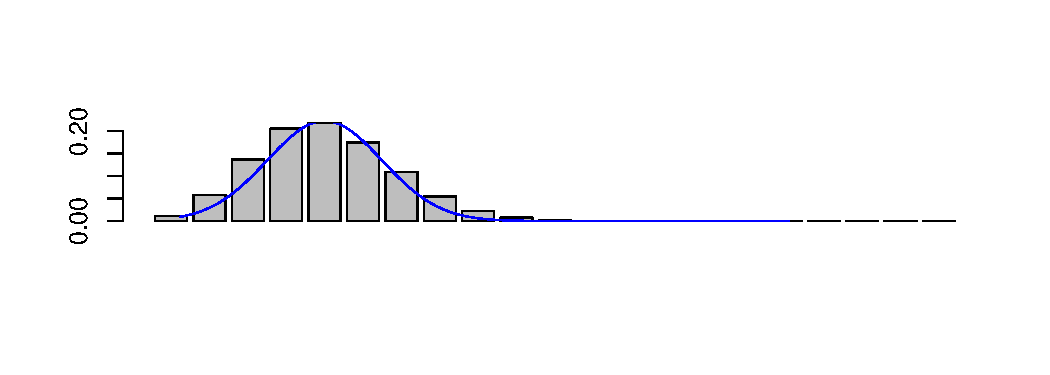
\includegraphics[width=\maxwidth]{figure/unnamed-chunk-9-1} 

\end{knitrout}

\begin{align*} 
P(X \geq 8) & \approx P(Y \geq 7.5) \\
& = P( \frac {Y - 4}{\sqrt(3.2)} \geq \frac{7.5-4}{\sqrt(3.2)} ) \\
& = P(Z \geq 1.956559 ) \\
& = 1-\Phi(1.956559) \\
& = 0.02519967
\end{align*}

\begin{knitrout}
\definecolor{shadecolor}{rgb}{0.969, 0.969, 0.969}\color{fgcolor}\begin{kframe}
\begin{alltt}
\hlnum{1}\hlopt{-}\hlkwd{pnorm}\hlstd{(}\hlnum{7.5}\hlstd{,}\hlnum{4}\hlstd{,}\hlkwd{sqrt}\hlstd{(}\hlnum{3.2}\hlstd{))}
\end{alltt}
\begin{verbatim}
## [1] 0.02519964
\end{verbatim}
\begin{alltt}
\hlnum{1}\hlopt{-}\hlkwd{pnorm}\hlstd{(}\hlnum{1.956559}\hlstd{)}
\end{alltt}
\begin{verbatim}
## [1] 0.02519967
\end{verbatim}
\end{kframe}
\end{knitrout}

\vspace{.5cm}
\item
Hence the absolute error is: $|0.03214266 -  0.02519967| = 0.00694299$. \\

The relative error of the approximation is $\frac{|0.03214266 -  0.02519967|}{0.03214266} = 0.2160055$. \\

A relative error of approximately 22\% indicates a poor approximation, but notice here the probabilities are small.
\end{parts}
\end{solution}




\newpage
\vspace{5cm} \hspace{-1cm} {\bf Extra Questions}

\question Sums of Random Variables \\

Given two random variables $X$: $E(X)=5$ and $Var(X)=9$ and $Y$: $E(Y)=3$ and $Var(Y)=4$. \\

\begin{parts}
\part Find $E(X+Y)$ and $Var(X+Y)$. What condition is necessary to calculate the variance?
\part Find $E(2X+Y+3)$ and $Var(2X+Y+3)$. 
\part Find $E(-5X-6Y)$ and $Var(-5X-6Y)$.
\end{parts}


\begin{solution}
(a) 
$E(X+Y) = E(X) + E(Y) = 5 + 3 = 8$ \\
$Var(X+Y) = Var(X) + Var(Y) = 9 + 4 = 13$ (assuming independence) \\

Condition: Independence of $X$ and $Y$. \\

(b)
$E(2X+Y+3) = 2E(X) + E(Y) + 3 = 2 \times 5 + 3 + 3 = 16$  \\
$Var(2X+Y+3) = 4Var(X) + Var(Y) = 4 \times 9 + 4 = 40$  \\

(c)
$E(-5X-6Y) = -5E(X) - 6E(Y) = -5 \times 5 -6 \times 3 = -43$ \\
$Var(-5X-6Y) = (-5)^2Var(X) + (-6)^2 Var(Y) = 25 \times 9 + 36 \times 4 = 369$ 
\end{solution}


\question Mean and Total of iid RVs \\

Suppose $X_{i} \sim N(100, 125)$ for $i=1,\ldots,5$.

\begin{parts}
\part Find the distribution of $\bar{X}$ and $T = \sum_{i=1}^{5} X_{i}$. 

\part Calculate $P(95 \leq \bar{X} \leq 105)$. Is this what you expected?

\part $P(T \geq 600)$. Is this what you expected?
\end{parts}


\begin{solution}
Given: $X_{i} \sim N(\mu = 100, \sigma^2= 125)$ for $i=1,\ldots,n$, where $n=5$. \\

(a) 
$\bar{X} \sim N(\mu, \frac{\sigma^2}{n} ) = N(100, \frac{125}{5} )  = N(100,25) = N(100, 5^2)$. \\

$T = \sum_{i=1}^{5} X_{i} \sim N( n \mu, n \sigma^2) = N(5 \times 100, 5 \times 125) = N(500, 625) = N(500, 25^2)$. \\

(b)
Standardising we get
\[  P(95 \leq \bar{X} \leq 105) = P(\frac{95-100}{5} \leq \frac{\bar{X} - 100}{5} \leq \frac{105-100}{5}) = P(-1 \leq Z \leq 1) \]
which is
\[  P(Z \leq 1) - P(Z \leq -1) = \Phi(1) - (1-\Phi(1)) = 2 \Phi(1) - 1 \approx 0.68  \]

This is what we expect: as 68\% of probability lies within 1 standard deviation of the mean. \\
 
(c)
Standardising we get
 \[ P(T \geq 600) = P( \frac{T - 500}{25} \geq \frac {600-500}{25})  = P( Z \geq 4) \approx 0 \]

This is what we expect: as it would be highly unlikely to observe a value more than 4 sds away from the mean.

\end{solution}








\question Central Limit Theorem \\

\begin{parts}

\part
In your own words, explain the Central Limit Theorem.

\part 
Why does the Central Limit Theorem apply to the Binomial Distribution?

\end{parts}


\begin{solution}
(a)
The Central Limit Theorem allows a {\it sum} of non-Normal random variables to be approximated by a Normal random variable. \\

(b)
The Binomial is a {\it sum} of Bernouli random variables.

\end{solution}




\question  Central Limit Theorem  \\

A new type of electronics flash for cameras will last an
average
    of 5000 hours with a standard deviation of 400 hours. A company
    quality control engineer intends to select a random sample of 100 of
    these flashes and use them until they fail.  \\

    \begin{parts}
    \part What is the approximate probability
    that the mean life time of 100 flashes will be less than 4940 hours?

    \part What is the approximate probability that the mean life time of 100 flashes will be between 4960 and 5040 hours (ie. within 40 hours of $\mu$, the population mean)
    \end{parts}


 \begin{solution}
Sample: Flash Lifetimes =  $X_{i} \sim N(5000, 400^2), i=1,2,\ldots, 100$. \\

(a)  
By the CLT,  $\bar{X} \rightarrow N( 5000, 400^2/100) = N( 5000, 40^2)$. \\

So \begin{align*}
 P( \bar{X}  < 4940)  & =  P( \frac{ \bar{X} - 5000}{40}  < \frac{4940-5000}{40} ) \\
& = P(Z < -1.5) \\
& = 1-\Phi(1.5) \\
& =  0.0668072
\end{align*}

\begin{knitrout}
\definecolor{shadecolor}{rgb}{0.969, 0.969, 0.969}\color{fgcolor}\begin{kframe}
\begin{alltt}
\hlkwd{pnorm}\hlstd{(}\hlnum{4940}\hlstd{,}\hlnum{5000}\hlstd{,}\hlnum{40}\hlstd{)}
\end{alltt}
\begin{verbatim}
## [1] 0.0668072
\end{verbatim}
\begin{alltt}
\hlnum{1}\hlopt{-}\hlkwd{pnorm}\hlstd{(}\hlnum{1.5}\hlstd{)}
\end{alltt}
\begin{verbatim}
## [1] 0.0668072
\end{verbatim}
\end{kframe}
\end{knitrout}

\vspace{.5cm}
(b)
 \begin{align*}
P( 4960 <      \bar{X}  < 5040) & = P( \frac{4960  - 5000}{40}  <     \frac { \bar{X} - 5000}{40}  < \frac{5040-5000}{40}) \\
& = P( -1 < Z < 1) \\
& = \Phi(1) - (1-\Phi(1)) \\
& = 2 \Phi(1) - 1 \\
& =  0.6826895 \\
\end{align*}
Note: This is as we expect - approximately 68\% chance of being 1 sd away from the mean.
\end{solution}


\question Combinations of Light Bulb Lifetimes \\

An electrical firm manufactures light bulbs. The lifetime of the bulbs is
approximately normally distributed, with average lifetime of 800 hours
and variance of 1600 hours. \\
                        

\begin{parts}
 \part
Find the probability that a randomly chosen light bulb lasts less than 790 hours.

\part
 Find the probability that the average lifetime of a sample of 25 bulbs is less than 790 hours.
                                        
  \end{parts}


\begin{solution}
$X = \text{lifetime of bulb} \sim N(800,1600)$. \\
                        
(a)
$P( X < 790) = P \big( \frac{X-800}{40} < \frac{790-800}{40} \big) = P(Z < -1/4) = P(Z > 1/4) = 1-\Phi(1/4) =0.4013$ \\

\begin{knitrout}
\definecolor{shadecolor}{rgb}{0.969, 0.969, 0.969}\color{fgcolor}\begin{kframe}
\begin{alltt}
\hlkwd{pnorm}\hlstd{(}\hlnum{790}\hlstd{,}\hlnum{800}\hlstd{,}\hlnum{40}\hlstd{)}
\end{alltt}
\begin{verbatim}
## [1] 0.4012937
\end{verbatim}
\end{kframe}
\end{knitrout}

\vspace{.5cm}
(b)
$\bar{X} = \text{average lifetime of bulb} \sim N(\mu, \sigma^2/n) = N(800,1600/25) = N(800,64)$. \\
 
$P( \bar{X} < 790) = P \big( \frac{\bar{X}-800}{8} < \frac{790-800}{8} \big) = P(Z < -10/8) = P(Z > 1.25) = 1-\Phi(1.25) =0.1056$ \\

\begin{knitrout}
\definecolor{shadecolor}{rgb}{0.969, 0.969, 0.969}\color{fgcolor}\begin{kframe}
\begin{alltt}
\hlkwd{pnorm}\hlstd{(}\hlnum{790}\hlstd{,}\hlnum{800}\hlstd{,}\hlnum{8}\hlstd{)}
\end{alltt}
\begin{verbatim}
## [1] 0.1056498
\end{verbatim}
\end{kframe}
\end{knitrout}
 \end{solution}





\question   Poor Normal approximation to Binomial \\

\begin{parts}
\part
Find the relative error of the Normal approximation to $P(X \leq 2)$, when $X \sim Bin(25,0.25)$.

\part
Can you explain why this is a poor appoximation?

\end{parts}



\begin{solution}
(a)
By the CLT, $X \rightarrow Y \sim N(6.25,4.6875)$. \\

As we are approximating a discrete distribution (Binomial) by a continuous distribution (Normal), we use a continuity correction and  change 2 to 2.5.
\begin{align*} 
P(X \leq 2) & \approx P(Y \leq 2.5) \\
& = P( \frac {Y - 6.25}{\sqrt{4.6875}} \leq \frac{2.5-6.25}{\sqrt{4.6875}} ) \\
& = P(Z \leq -1.732051 ) \\
& = 1-\Phi(1.732051) \\
& = 0.04163224
\end{align*}

(b)
Exact probability is 0.03210852.
\begin{knitrout}
\definecolor{shadecolor}{rgb}{0.969, 0.969, 0.969}\color{fgcolor}\begin{kframe}
\begin{alltt}
\hlkwd{pbinom}\hlstd{(}\hlnum{2}\hlstd{,}\hlnum{25}\hlstd{,}\hlnum{0.25}\hlstd{)}
\end{alltt}
\begin{verbatim}
## [1] 0.03210852
\end{verbatim}
\end{kframe}
\end{knitrout}

Hence the relative error of approximation is $\frac{0.03210852 -  0.04163224}{0.03210852} = -0.2966104$. \\

A relative error of approximately 30\% indicates a poor approximation.  \\

(c)
This is surprising given that the `Guide' is satisfied, which reminds us that the `Guide' is merely a rule of thumb.
\end{solution}

\question Normal approximation to Discrete RV \\

Let $X_1,X_2,X_3$ be independent rolls of a fair 6-sided die and let
$S=X_1+X_2+X_3$. \\

\begin{parts}
\part
Show that $E(X_i)=3.5$ and Var$(X_i)=\frac{35}{12}$.

\part 
Compute a normal approximation with continuity correction for $P(S\leq 6)$.

\part 
Using probability, compute $P(S\leq 6)$ exactly. What is the relative error of the approximation in (b)?

\end{parts}
                                    

\begin{solution}
Let $X_1,X_2,X_3$ be independent rolls of a fair 6-sided die and let
$S=X_1+X_2+X_3$. \\

(a)
Let $X_{i} = i\text{th toss of a fair die}$, $i=1,2,3$. \\

\begin{tabular}{|l |l |l |l |l |l |l |l  |} \hline
$x_{i}$ & 1   & 2  & 3  & 4 & 5 & 6 &  Total \\ \hline
$P(X_{i} = x_{i})$ & 1/6 &1/6 &1/6 &1/6 &1/6 &1/6 & 1 \\ \hline
\end{tabular}

\vspace{.5cm}
Then: \\
$E(X_i)= 1 \times 1/6 + 2 \times 1/6 + \ldots 6 \times 1/6 = 3.5$ \\
$E(X_i^2)= 1^2 \times 1/6 + 2^2 \times 1/6 + \ldots 6^2 \times 1/6 = 91/6$ \\
$Var(X_i)=91/6 - 3.5^2 = 35/12$ \\

(b)
By the CLT,  $S = \sum_{i=1}^{3} X_{i} \rightarrow Y \sim N( 3 \times 3.5, 3 \times 35/12) = N( 10.5, 8.75)$. \\

As we are approximating a discrete distribution by a continuous distribution (Normal), we use a continuity correction and  change 6 to 6.5.
\begin{align*} 
P(S \leq 6) & \approx P(Y \leq 6.5) \\
& = P( \frac {Y - 10.5}{\sqrt{8.75}} \leq \frac{6.5-10.5}{\sqrt{8.75}} ) \\
& = P(Z \leq -1.352247) \\
& = 1-\Phi(1.352247) \\
& =0.08814816
\end{align*}

\vspace{.5cm}
(c)
Consider the number of ways to get a total of 6: 
$\{ 111, 112, 113, 114, 121 ... 222\}$, altogether there are 20 ways, and each has a probability of $\frac{1}{6^3}$. \\
Hence 
$P(S\leq 6) = \frac{20}{6^3} \approx 0.093 $. \\
Hence the relative error of approximation in (b) is $\frac{\frac{20}{6^3} - 0.08814816}{\frac{20}{6^3}} = 0.04799987$. \\
A relative error of approximately 5\% is excellent, given we are approximating a discrete sum of only 3 variables.

\end{solution}


\question  Normal Approximation to Binomial \\

Suppose that $X\sim B(20,0.25)$. \\

\begin{parts}
  \part Write down $E(X)$ and $Var(X)$.
\part Compute a normal approximation to $P(X\geq5)$ using a continuity correction.
\part Use R to compute the exact probability. What is the relative error of the approximation in (b).
\part Repeat (a)-(c) for $X\sim B(20,0.1)$.
\part Why is the relative error in (d) so poor compared to (c)?
\end{parts}



\begin{solution}
(a)  $E(X) = np = 5$ and $Var(X)=np(1-p)=3.75$. \\

(b)
By the CLT, $X \sim Bin(20,0.25) \rightarrow Y \sim N(5,3.75)$. \\

As we are approximating a discrete distribution (Binomial) by a continuous distribution (Normal), we use a continuity correction and  change 5 to 4.5.
\begin{align*} 
P(X \geq 5) & \approx P(Y \geq 4.5) \\
& = P( \frac {Y - 5}{\sqrt{3.75}} \geq \frac{4.5-5}{\sqrt{3.75}} ) \\
& = P(Z \geq -0.2581989 ) \\
& = \Phi(0.2581989) \\
& = 0.6018733
\end{align*}

\vspace{.5cm}
(c)
\begin{knitrout}
\definecolor{shadecolor}{rgb}{0.969, 0.969, 0.969}\color{fgcolor}\begin{kframe}
\begin{alltt}
\hlnum{1}\hlopt{-}\hlkwd{pbinom}\hlstd{(}\hlnum{4}\hlstd{,}\hlnum{20}\hlstd{,}\hlnum{0.25}\hlstd{)}
\end{alltt}
\begin{verbatim}
## [1] 0.5851585
\end{verbatim}
\end{kframe}
\end{knitrout}

Hence the relative error of approximation in (a) is $\frac{0.5851585 -  0.6018733}{0.5851585} = -0.02856457$. \\
A relative error of approximately 3\% again reflects an accurate approximation. \\

(d)
Given $X\sim B(20,0.1)$, $E(X) = np = 2$ and $Var(X)=np(1-p)=1.8$. \\

By the CLT, $X \rightarrow Y \sim N(2,1.8)$. \\

As we are approximating a discrete distribution (Binomial) by a continuous distribution (Normal), we use a continuity correction and  change 5 to 4.5.
\begin{align*} 
P(X \geq 5) & \approx P(Y \geq 4.5) \\
& = P( \frac {Y - 2}{\sqrt{1.8}} \geq \frac{4.5-2}{\sqrt{1.8}} ) \\
& = P(Z \geq 1.86339 ) \\
& = 1-\Phi(1.86339) \\
& = 0.03120371
\end{align*}

Exact probability is 0.0431745.
\begin{knitrout}
\definecolor{shadecolor}{rgb}{0.969, 0.969, 0.969}\color{fgcolor}\begin{kframe}
\begin{alltt}
\hlnum{1}\hlopt{-}\hlkwd{pbinom}\hlstd{(}\hlnum{4}\hlstd{,}\hlnum{20}\hlstd{,}\hlnum{0.1}\hlstd{)}
\end{alltt}
\begin{verbatim}
## [1] 0.0431745
\end{verbatim}
\end{kframe}
\end{knitrout}

Hence the relative error of approximation is $\frac{0.0431745 -  0.03120371}{0.0431745} = 0.2772653$. \\
A relative error of approximately 28\% indicates a very poor approximation.  \\

(e) Comparing $Bin(20,0.1)$ to the `Guide' for using Normal approximation, we find that $np <5$ and $n(1-p)  >5$, hence it is not surprising that the approximation is not accurate.
\end{solution}

\question Sum of iid Normal Random Variables \\

Suppose that the weight (in pounds) of a North American
adult can be represented by a normal random variable with mean
150 and variance 625. An elevator contains a sign ``Maximum 10 people". It can in fact safely carry 2000 lbs. \\
                        
\begin{parts}

\part (Extension) If we want to be at least 99\% certain that the elevator will not be
overloaded, what is the maximum number of people that should be
allowed into the elevator?

\part If we want an elevator that we are 99\% certain can carry 10 people without overloading, how much weight
should it be able to safely carry?
\end{parts}


%\newpage
\begin{solution}

$X_{i} = \text{weight of a North American
adult} \sim N(150,625)$, $i=1,2,\ldots,n$\\

Safety limit for the lift: \\
Sign says: `Maximum 10 people'  \\
Actual limit: 2000 pounds \\
                        
(a)
We want to find $n$ such that $P(\text{total weight $\leq$  safety limit}) = P(\sum_{i=1}^{n} X_{i} \leq 2000) \geq 0.99$. \\

Now $\sum_{i=1}^{n} X_{i} \sim N( n \mu, n \sigma^2) 
= N( 150n, 625n)$. \\

So $P( \sum_{i=1}^{n} X_{i} \leq 2000)  = P \big( \frac{
\sum_{i=1}^{n} X_{i} - 150n}{25\sqrt{n}} \leq \frac{
2000 - 150n}{25\sqrt{n}} \big) = P(Z \leq \frac{
2000 - 150n}{25\sqrt{n}} ) $ \\

Hence we want to find $n$ such that
$P(Z \leq \frac{ 2000 - 150n}{25\sqrt{n}} ) \geq 0.99$. \\
\\

From the Normal table, the 99\% quantile of $Z$ is 2.33. \\

Hence we need to solve $\frac{ 2000 - 150n}{25\sqrt{n}} \geq 2.33$. \\

(1) Method1: Using quadratic \\
Rearranging, we get $150n +58.25 \sqrt{n} -2000 = 0$, 
which is a quadratic in $\sqrt{n}$. \\

Using the quadratic formula, \\
$\sqrt{n} = \frac{ -58.25 \pm \sqrt{58.25^2- 4 \times 150 \times -2000}}{2 \times 150}$ \\
so $\sqrt{n}$ = $-3.850809$ or $3.462476$,
giving $n = (3.462476)^2 = 11.98874$. \\
Hence, we would choose $n=11$ to be safe. \\

(2) Method2: Using trial and error \\

\begin{tabular}{|l|c|} \hline
$n$ & $\frac{2000 - 150n}{25\sqrt{n}}$ \\ \hline
9 &  8.7 \\
10 & 6.3 \\
11 &  4.2 \\
12 & 2.3 \\
13 & 0.6 \\ \hline
\end{tabular}

\vspace{.2cm}
To get $\frac{2000 - 150n}{25\sqrt{n}} \geq 2.33$, we need a maximum of $n =11$. \\


(b) 
We want to find $L$ such that $P(\sum_{i=1}^{10} X_{i} \leq L) \geq 0.99$. \\

Now $\sum_{i=1}^{10} X_{i} \sim N( 1500, 6250)$. \\

So $P( \sum_{i=1}^{10} X_{i} \leq L)  = P \big( \frac{
\sum_{i=1}^{10} X_{i} - 1500}{\sqrt{6250}} \leq \frac{
L - 1500}{\sqrt{6250}} \big) = P(Z \leq \frac{
L - 1500}{\sqrt{6250}} ) $ \\

Hence we want $P(Z \leq \frac{
L - 1500}{\sqrt{6250}} )  \geq 0.99$.

Solving $2.33 = \frac{
L - 1500}{\sqrt{6250}}$, we get
$L = 2.33*\sqrt{6250} + 1500 = 1684.203$. \\
Hence, choose a safety limit of 1684 pounds.
\end{solution}

\question A pharmaceutical firm produces a rare antibiotic. It is believed that
daily production (in mg) of the drug may be represented by a normal random
variable with mean 500 and variance 1600.  \\

\begin{parts}
\part 
A hospital wants as much of the antibiotic as possible five weeks
from now. Assuming independence of the production each day and 5
working days per week, how much of the antibiotic can the firm
promise, and be 90\% certain of keeping its promise?

\part (Extension)
After delivering the antibiotic to the hospital, the firm receives
an urgent order for 10 grams of the drug from a hospital in
Iqaluit. How quickly can the hospital promise to deliver the
order, and be 95\% certain of keeping its promise?
 \part After studying its production more closely, the firm realizes
that its production (in mg/day) varies due to absenteeism. The
daily means  and variances  are as follows:\\ 

\begin{center}
\begin{tabular}{| l|l|l | } \hline
Day& Mean& Variance\\\hline
Monday&300&900\\
Tuesday&500&1000\\
Wednesday&600&1100\\
Thursday&500&1000\\
Friday&300&900 \\ \hline
\end{tabular}
\end{center}

If it can be assumed that each day's production is normally
distributed and independent of the other days, what is the
probability that the total production in a week exceeds 2 grams?

\part Verify your answers in (a) and (c) by using the R commands \texttt{pnorm} and \texttt{qnorm}.
\end{parts}


\begin{solution}
Daily Production $= X_{i} \sim N(500,1600), i=1,2,3, \ldots$ \\

(a)
Total production in 25 days = $\sum_{i=1}^{25} X_{i} \sim N(25 \times 500,25 \times 1600) = N(12500,200^2)$ \\

We want $L$ such that $P(\sum_{i=1}^{25} X_{i} \geq L) \geq 0.90$.  \\

Hence $P(\frac{ \sum_{i=1}^{25} X_{i} - 12500}{200} \geq \frac{L-12500}{200}) \geq 0.90$. \\

\vspace{.5cm}
Solving $-1.28 = \frac{L-12500}{200}$, we get
$L = -1.28 \times 200 + 12500 = 12244$.

Hence, the firm could promise a production of 12244g. \\


(b)
We want $n$ (number of days) such that $P(\sum_{i=1}^{n} X_{i} \geq 10000) \geq 0.95$.  \\

Total production in $n$ days = $\sum_{i=1}^{n} X_{i} \sim N(500n,1600n)$ \\

So we want $P(\sum_{i=1}^{n} X_{i} \geq 10000)
= P(\frac{ \sum_{i=1}^{n} X_{i} - 500n}{\sqrt{1600n}} \geq \frac{ 10000-500n}{\sqrt{1600n}} )
 = P(Z \geq \frac{ 10000 -500n}{\sqrt{1600n}} )
\geq 0.95$ \\

\vspace{.5cm}
We need to solve $-1.645 = \frac{ 10000 -500n}{\sqrt{1600n}}$. \\

(1) Method1: Using quadratic \\
Rearranging gives the quadratic in $\sqrt{n}$: $500n -65.8 \sqrt{n} - 10000 = 0$. \\

Using the quadratic formula, we get
$\sqrt{n} = \frac{ 65.8 \pm \sqrt{-65.8^2- 4 \times 500 \times -10000}}{2 \times 500}$ \\
which gives $\sqrt{n} = -4.40682$ and $4.53842$.

Hence $n= 21$. The hospital expects to deliver within 21 days. \\

(2) Method2: Using trial and error \\

\begin{tabular}{|l|c|} \hline
$n$ & $\frac{10000 -500n}{\sqrt{1600n}}$ \\ \hline
19 &  2.867697 \\
20 & 0 \\
21 & -2.727724 \\ 
22 & -5.330018 \\ \hline
\end{tabular}

\vspace{.2cm}
To get $\frac{10000 -500n}{\sqrt{1600n}} \geq 1.645$, we need a maximum of $n =21$. \\



(c)
Total Production in a week = $T \sim N( 300 + 500 + 600 +500 + 300, 900+1000+1100+1100+900)$. \\
So $T \sim N(2200, 5000)$.

Hence $P( T \geq 2000) = P( \frac{T-2200}{\sqrt{5000}} \geq \frac{2000=2200}{\sqrt{5000}})
= P(Z \geq -2.828427) \doteq 0.998$ \\

(d)
\begin{knitrout}
\definecolor{shadecolor}{rgb}{0.969, 0.969, 0.969}\color{fgcolor}\begin{kframe}
\begin{alltt}
\hlkwd{qnorm}\hlstd{(}\hlnum{0.1}\hlstd{,}\hlnum{12500}\hlstd{,}\hlnum{200}\hlstd{)}
\end{alltt}
\begin{verbatim}
## [1] 12243.69
\end{verbatim}
\begin{alltt}
\hlnum{1}\hlopt{-}\hlkwd{pnorm}\hlstd{(}\hlnum{2000}\hlstd{,}\hlnum{2200}\hlstd{,}\hlnum{70}\hlstd{)}
\end{alltt}
\begin{verbatim}
## [1] 0.9978626
\end{verbatim}
\end{kframe}
\end{knitrout}

\end{solution}














\end{questions}

\end{tutorial}
\end{document}


